\chapterA{Diseño combinacional avanzado}
\section{Módulos combinacionales}

\subsection{Decodificador}
Circuito combinacional con n entradas y $2^{n}$ salidas. Cada salida es uno de los minterms que pueden generarse con n variables.
\[
    D_{i} =\left\{ \begin{array}{l}
        1\; si\; A=i donde\; A= \sum^{n-1}_{j=0}A_{j}2^{j}\; para\; 0 \leq i \leq 2^{n} -1 \\
        0 \; en \; caso \; contrario
    \end{array}\right\}
\]

\begin{figure}[H]
    \centering
    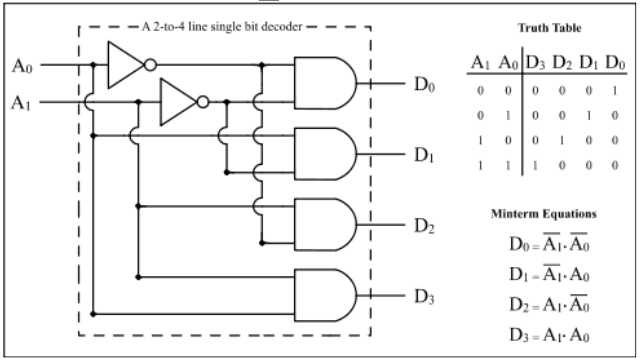
\includegraphics[width=0.8\textwidth]{images/Tema_3/Decodificador.PNG}
\end{figure}
\begin{figure}[H]
    \centering
    \lstinputlisting[style=customVHDL,  xleftmargin=.2\textwidth, xrightmargin=.2\textwidth]{Code/Tema_3/Decodificador.vhd}
\end{figure}

\subsection{Decodificador}
\begin{figure}[H]
    \centering
    \lstinputlisting[style=customVHDL,  xleftmargin=.2\textwidth, xrightmargin=.2\textwidth]{Code/Tema_3/Codificador.vhd}
\end{figure}

\subsection{Multiplexor}

Descripción de alto nivel:
\[
    y = x_{s} \; donde \; s=\sum^{n-1}_{j=0} x_{j}2^{j}
\]

Implementación
\begin{itemize}
    \item 2 a 1 $y = x_{0} * \overline{s} + x_{1} * s$
    \item 4 a 1 $y = x_{0}\,\overline{s_{1}}\,\overline{s_{0}} + x_{1}\,\overline{s_{1}} \,s_{0} + x_{2}\,s_{1}\,\overline{s_{0}} + x_{3}\,s_{1}\,s_{0}$
\end{itemize}

\begin{figure}[H]
    \centering
    \lstinputlisting[style=customVHDL,  xleftmargin=.2\textwidth, xrightmargin=.2\textwidth]{Code/Tema_3/Multiplexor.vhd}
\end{figure}
\newpage
\subsection{Sumador}
\begin{multicols}{2}
    \begin{figure}[H]
        \centering
        \lstinputlisting[style=customvhdl]{Code/Tema_3/Sumador1.vhd}
        \caption{Sumador con std\_logic}
    \end{figure}
    \vfill
    \null
    \begin{figure}[H]
        \centering
        \lstinputlisting[style=customvhdl]{Code/Tema_3/Sumador2.vhd}
        \caption{Sumador con numeric y datos con signo}
    \end{figure}
\end{multicols}

\begin{figure}[H]
    \centering
    \lstinputlisting[style=customvhdl]{Code/Tema_3/Restador.vhd}
    \caption{Restador}
\end{figure}


\section{Aritmética en VHDL}
\subsection{Operadores incluidos en VHDL-93 sin incluir ningún paquete}
